In this part of the document we'll talk about the Hennessy-Milner
logic over CCS processes. We approach the logic in two steps: the
former without recursion, where we'll use the logic to show the
non-bisimilarity of toy processes; the latter including recursion
operators, where we'll build a simple model involving a car and a
train, aiming to verify some safety and liveness properties.

\section{$\mu$-calculus definition}
Following \cite{MuScSt1999}, $\mu$-calculus formulae are constructed
according to the following grammar:
\begin{displaymath}
  \phi := tt \mid ff \mid \phi_1 \wedge \phi_2 \mid \phi_1 \vee \phi_2 \mid
  \langle a \rangle \phi \mid [a]\phi \mid X \mid \mu X.\phi
  \mid \nu X.\phi
\end{displaymath}
where $a \in Act$, $X \in Var$, $tt$ means \emph{true} and $ff$ means
\emph{false}. The fix point operators $\mu X.\phi, \nu X.\phi$ bind
free occurrences of variable $X \in Var$.

Formulae that can be composed using the syntax above are interpreted
over \emph{Labeled Transition Systems}. Given an \emph{Labeled
  Transition Systems} $T = (S, Act, \rightarrow)$, we interpret a
\emph{closed} formula $\phi$ as the subset of states whose make $\phi$
true while we interpret an \emph{open} formula using a function (also
called \emph{environment}) $\rho$ such that $\rho: Var \rightarrow
2^S$. Roughly speaking, $\rho(X)$ interprets a free variable $X$
contained in a formula $\phi$ by a subset of $S$, representing an
assumption about the set of states satisfying the sub formula $X$.

Let $T = (S, Act, \rightarrow)$ be a \emph{Labeled Transition
  Systems}, $\phi$ a formula and $\rho$ an environment, we define the
set $\mathcal{M}_T(\phi, \rho) \subseteq S$ satisfying $\phi$ is
defined inductively as follows:
\begin{displaymath}
  \begin{split}
    \mathcal{M}_T(tt, \rho) &= S \\
    \mathcal{M}_T(ff, \rho) &= \emptyset \\
    \mathcal{M}_T(\phi_1 \wedge \phi_2, \rho) &=
    \mathcal{M}_T(\phi_1, \rho) \cap     \mathcal{M}_T(\phi_2, \rho)\\
    \mathcal{M}_T(\phi_1 \vee \phi_2, \rho) &=
    \mathcal{M}_T(\phi_1, \rho) \cup     \mathcal{M}_T(\phi_2, \rho)\\
    \mathcal{M}_T([a]\phi, \rho) &= \{ s\in S: \forall s^{\prime}: s
    \xrightarrow{a} s^{\prime} \rightarrow s^{\prime} \in
    \mathcal{M}_T(\phi, \rho)\} \\
    \mathcal{M}_T(\langle a \rangle \phi, \rho) &= \{ s\in S: \exists
    s^{\prime}: s \xrightarrow{a} s^{\prime} \wedge s^{\prime} \in
    \mathcal{M}_T(\phi, \rho)\} \\
    \mathcal{M}_T(X, \rho) &= \rho(X) \\
    \mathcal{M}_T(\mu X.\phi, \rho) &= fix_{\mu}F_{\phi, \rho, X} \\
    \mathcal{M}_T(\nu X.\phi, \rho) &= fix_{\nu}F_{\phi, \rho, X} \\
  \end{split}
\end{displaymath}
where $fix_{\mu}F_{\phi, \rho, X}, fix_{\nu}F_{\phi, \rho, X}$ mean
the least and greater fixed points of the function $F_{\phi, \rho, X}:
2^S \rightarrow 2^S$, which is defined as:
\begin{displaymath}
  F_{\phi, \rho, X}(x) = \mathcal{M}_T(\phi, \rho_{X, x, \rho}^{\prime})
\end{displaymath}
where $\rho_{X, x, \rho}^{\prime}: Var \rightarrow 2^S$ is defined as:
\begin{displaymath}
  \begin{split}
    \rho_{X, x, \rho}^{\prime}(X) &= x \\
    \rho_{X, x, \rho}^{\prime}(Y) &= \rho(Y) \quad \text{if } X\not=Y\\
  \end{split}
\end{displaymath}

Let $T = (S, Act, \rightarrow)$ be a finite-state \emph{Labeled
  Transition Systems} (those for the set of states is finite), due to
\emph{Kleene fix point theorem} it is possible to characterize $
\mathcal{M}_T(\mu X.\phi, \rho)$ and $ \mathcal{M}_T(\nu X.\phi,
\rho)$ by the following identities:
\begin{displaymath}
  \begin{split}
    \mathcal{M}_T(\mu X.\phi, \rho) = \bigcup \{F_{\phi, \rho,
      X}^i(\emptyset):i\geq 0\} \\
    \mathcal{M}_T(\nu X.\phi, \rho) = \bigcap \{F_{\phi, \rho,
      X}^i(S):i\geq 0\} \\
  \end{split}
\end{displaymath}
where $F_{\phi, \rho, X}^{i+1}(a) = F_{\phi, \rho, X}(F_{\phi, \rho,
  X}^i(a))$ and $F_{\phi, \rho, X}^0(a) = a$.

\section{Model checker implementation}

In this section we describe our implementation of a \emph{local model
  checker} using the programming language OCaml. The development of
the module has been structured in the following way:
\begin{enumerate}
\item built a new type $Process$ with the necessary constructors to
  make \emph{CCS processes};
\item built a function $unfold\_process$ which allow to do one
  ``unfolding step'' respect to a free variable $X$ bound by a $Recur$
  process constructor;
\item built a function $next$ which consume a $Process$ and return a
  list of of possible computations that the given process exhibits;
\item built a new type $formula$ with the necessary constructors to
  make $\mu$-calculus formulae;
\item built a function $unfold\_formula$ which allow to do one
  ``unfolding step'' respect to a free variable $X$ bound by a fix
  point operator;
\item built a function $sat$ which consume a process $p$ and a formula
  $f$ and produce the decision of $p \vdash f$, if $p$ is a finite
  state process.
\end{enumerate}

We would like to discuss briefly the details of function $sat$. This
is the core of the model checker, using a local strategy explained in
the Winskel's work \cite{Winskel1991157}. It is a bit different
respect the theory described above because a nice idea is introduced
for fix point operators: Winskel allow a free variable to curry a set
a states in a recursive formula specification, for example it is
possible to write the formula $\nu X\{p_1,\ldots,p_n\} A$, where $p_i
\in S$ and $A$ is a $\mu$-calculus formula (where the $X$ variable
probably occur into it). This is important due the following
equivalence:
\begin{displaymath}
  p \in \nu X.\gamma(X) \leftrightarrow p \in \gamma (\nu X(\{p\}\cup\gamma(X)))
\end{displaymath}
where $\gamma : 2^S \rightarrow 2^S$ monotonic respect set inclusion
relation. Roughly speaking, the equivalence says that the process $p$
satisfies the recursively defined formula if and only if $p$ satisfies
a certain kind of unfolding of the recursively defined
formula. Winskel asks to proof the following statement which is
directly implemented in our implementation of $sat$ function:
\begin{displaymath}
  p \in \left \lbrace p_1,\ldots,p_n\right\rbrace \rightarrow
  p \vdash \nu X \left \lbrace p_1,\ldots,p_n\right\rbrace A
\end{displaymath}

\begin{proof}
  By contropositive, writing $\nu X \left \lbrace
    p_1,\ldots,p_n\right\rbrace A$ as $\nu X (\left \lbrace
    p_1,\ldots,p_n\right\rbrace \vee A)$ and $\cdot[ \frac{T}{X} ]$ is
  a function (written in post fix notation) such that $[ \frac{T}{X} ]:
  2^S \rightarrow 2^S$, we have:
  \begin{displaymath}
    \begin{split}
      p & \not \vdash \nu X (\left \lbrace p_1,\ldots,p_n\right\rbrace
      \vee A) \\
      & \updownarrow \text{ by def of relation } \vdash  \\
      p & \not \in \bigcup\left\{T \in 2^S: T\subseteq (\left \lbrace
          p_1,\ldots, p_n \right\rbrace \cup A )\left[ \frac{T}{X} \right] \right\}\\
      & \updownarrow \\
      \not \exists T \in (2^S \setminus \emptyset)&:T \subseteq (\left
        \lbrace p_1,\ldots, p_n \right\rbrace \cup A)\left[
        \frac{T}{X} \right] \quad \text{ such that } \quad p \in T \\
      & \updownarrow \left \lbrace p_1,\ldots, p_n \right\rbrace
      \text{ cannot contain free occurrences of } X \in Var  \\
      \not \exists T \in (2^S \setminus \emptyset)&:T \subseteq \left
        \lbrace p_1,\ldots, p_n \right\rbrace \cup A\left[
        \frac{T}{X} \right] \quad \text{ such that } \quad p \in T \\
      & \updownarrow \text{ in particular } T = \left \lbrace
        p_1,\ldots, p_n \right\rbrace \text{doesn't satisfy
        the condition} \\
      p &\not\in \left \lbrace p_1,\ldots, p_n \right\rbrace
    \end{split}
  \end{displaymath}
 
\end{proof}

\section{Case studies}

In this section we report two models that we've checked using our
implementation described in the section above.

\subsection{Non-bisimilar processes}

The processes under study are taken from \cite{1324845} and are
reported in \autoref{fig:not-bisimilar-processes}. Those processes
aren't bisimilar pairwise and, using the result that two processes are
bisimilar if and only if they satisfy exactly the same formulae, we
exhibit three witnesses of non-bisimilarity:
\begin{figure}[htb]
  \centering
  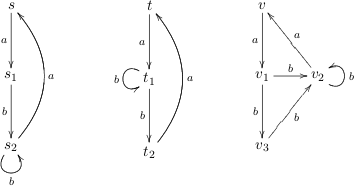
\includegraphics{qualitative-project/not-bisimilar-processes.png}
  \caption{Three not bisimilar processes}
  \label{fig:not-bisimilar-processes}
\end{figure}

\begin{verbatim}
Process s: RecX(a?.b?.RecY((b?.Y + a?.X)))
Process t: RecX(a?.RecY((b?.Y + b?.a?.X)))
Process v: RecX(a?.(b?.b?.RecY((b?.Y + a?.X)) + b?.RecY((b?.Y + a?.X))))

s isn't  bisimilar to t due to formula f= [a][b]<a>tt
s satisfy f: true
t satisfy f: false

s isn't  bisimilar to v due to formula f= [a]<b>[a]ff
s satisfy f: false
v satisfy f: true

t isn't  bisimilar to v due to formula f= [a]<b>[b]ff
t satisfy f: true
v satisfy f: false
\end{verbatim}

\subsection{Car-train crossing}

In this model we catch the situation of a cross between a road and a
rail. On both tracks a vehicle attempts to cross, a car and a train
respectively. In order to cross, a vehicle have to synchronize with a
``semaphore''.

We build the necessary \emph{CCS processes} in order to implement the
model and we proceed to verify the following properties:
\begin{itemize}
\item a train eventually cross, written in $\mu$-calculus using a min
  fix point:
  \begin{displaymath}
    \mu Z(\langle train\_cross\rangle tt \vee \langle Act
    \rangle Z)
  \end{displaymath}
\item it is no possible for the car and the train to cross
  simultaneously, written in $\mu$-calculus using a max fix point:
  \begin{displaymath}
    \nu Z(([train\_cross]ff \vee [car\_cross]ff) \wedge [Act]Z)
  \end{displaymath}
\item for each car $c$ that attempts to cross, $c$ eventually succeed,
  written in $\mu$-calculus using a mixture of min and max fix points:
  \begin{displaymath}
    \nu Z([car](\mu Y(\langle Act \rangle tt \vee [-car\_cross]Y))
    \wedge  [-car]Z)
  \end{displaymath}
  It is interesting to note that the above formula does not use
  \emph{alternating fix points}, that is the variable $Z$ bound by the
  out most $\nu$ does not appear in the context of the formula bounded
  by the innermost $\mu$. This is not the worst case for the
  $\mu$-calculus model checking (it is possible to write an equivalent
  \emph{aCTL} formula for the above one using the ``infinitely often''
  templates, while a formula with \emph{alternating fix points} has
  not an \emph{aCTL} equivalent).
\end{itemize}
Those properties are liveness, safety and fairness properties and
involve the solution of a min fixed point, a max fixed point and a
mixture of min and max fixed points respectively. We've written those
properties using our OCaml formula constructors and verified them with
the following results:
\begin{verbatim}
Process road: RecX(car?.up?.car_cross!.down!.X)
Process rail: RecY(train?.green?.train_cross!.red!.Y)
Process signal: RecZ((green!.red?.Z + up!.down?.Z))
Process crossing: (((RecX(car?.up?.car_cross!.down!.X) |
RecY(train?.green?.train_cross!.red!.Y)) | RecZ((green!.red?.Z +
up!.down?.Z))))\{green, red, up, down}
(((RecX(car?.up?.car_cross!.down!.X) |
RecY(train?.green?.train_cross!.red!.Y)) | RecZ((green!.red?.Z +
up!.down?.Z))))\{green, red, up, down}
Process crossing satisfy maxZ(([train_cross]ff or [car_cross]ff)
                                  and [Act]Z): true
Process crossing satisfy minZ(<train_cross>tt or <Act>Z): true
Process crossing satisfy maxZ([car](minY(<Act>tt and [-car_cross]Y))
                                  and  [-car]Z): true
\end{verbatim}
